\chapter{Appendice}
\section{Guida nell'analisi dell'incertezza secondo l'EFSA}

Il comitato scientifico dell'Autorità europea per la sicurezza alimentare (EFSA) ha sviluppato una guida dettagliata\footcite{womak:guida-analisi-incertezza} sull'analisi dell'incertezza nelle valutazioni scientifiche, con l'obiettivo di fornire una base solida per il processo decisionale in situazioni di incertezza.\\
Tale comitato è composto da eminenti scienziati di tutta Europa, ciascuno con una comprovata eccellenza scientifica e una vasta esperienza in varie discipline rilevanti per il mandato dell'EFSA. Tra le loro competenze si annoverano la valutazione dei rischi per la salute umana, l'epidemiologia, la microbiologia, la nutrizione umana, la chimica, la biologia e molte altre aree scientifiche. Questo gruppo multidisciplinare lavora per sviluppare metodologie armonizzate di valutazione del rischio e per garantire l'omogeneità dei pareri scientifici.\\
Le questioni affrontate dal comitato sono spesso di natura multidisciplinare, richiedendo approcci innovativi e integrati per la valutazione del rischio. Tra queste, vi sono l'armonizzazione dell'uso di ipotesi predefinite in assenza di dati reali.\\

Secondo tale comitato, l'analisi dell'incertezza nelle valutazioni scientifiche varia a seconda della natura della valutazione stessa. È essenziale identificare il tipo di valutazione in corso per poi seguire le linee guida specifiche.\\

\noindent Tipologie di Valutazione:
\begin{itemize}
    \item Valutazioni standardizzate: Queste seguono procedure prestabilite e dettagliate, spesso utilizzate per prodotti regolamentati come le autorizzazioni di preimmissione sul mercato. Queste procedure richiedono dati da studi specifici e includono criteri e calcoli standardizzati.
    \item  Valutazioni specifiche per il caso in esame: Necessarie quando non esistono procedure standardizzate. I valutatori devono sviluppare un piano di valutazione personalizzato, utilizzando elementi standardizzati dove possibile ma adottando approcci specifici per altre parti.
    \item  Elaborazione o revisione di documenti orientativi: Coinvolge la creazione o l'aggiornamento di procedure standardizzate.
    \item  Valutazioni urgenti: Richiedono completamento rapido con risorse limitate e implicano approcci semplificati.
    
\end{itemize}

In alcune aree dell'EFSA, una valutazione standardizzata può evidenziare la necessità di un'analisi più approfondita. In questi casi, si passa a una valutazione specifica per il caso, sostituendo elementi standardizzati con approcci su misura.\\
Le valutazioni possono essere quantitative (stima di una quantità) o qualitative (risposta verbale a una domanda). Anche se una valutazione è qualitativa, le conclusioni devono essere ben definite. L'incertezza può essere espressa quantitativamente tramite probabilità, pertanto, è raccomandato che i valutatori cerchino di quantificare l'incertezza anche quando utilizzano metodi qualitativi, poiché i metodi qualitativi hanno comunque un ruolo importante nell'analisi dell'incertezza.\\

% \subsection{Analisi dell'incertezza per le valutazioni standardizzate}
Quando si analizza l'incertezza in una valutazione standardizzata, è cruciale distinguere tra incertezze standard e non standard. Prima di tutto, bisogna determinare se esistono incertezze non standard. Se non ci sono, basta riportare che la valutazione non presenta incertezze non standard. In caso contrario, bisogna valutare l'impatto di queste incertezze sul risultato della procedura standard. Se l'incertezza non standard è significativa, potrebbe essere necessario passare a una valutazione specifica per il caso in esame.\\

% \subsection{Analisi dell'incertezza per valutazioni specifiche per il caso in esame}

Per le valutazioni specifiche per il caso, i valutatori devono seguire istruzioni pertinenti e, se necessario, consultare pareri scientifici di supporto. Dopo aver pianificato la valutazione e identificato le incertezze, bisogna decidere se suddividere l'analisi dell'incertezza in parti. Questa scelta dipende dalle domande e quantità rilevanti per la valutazione. \\
Valutare le incertezze collettivamente è il metodo più semplice, dove tutte le incertezze vengono valutate insieme nell'ambito della valutazione specifica.

Se l'analisi richiede risposte a domande sì/no, i valutatori possono esprimere le incertezze utilizzando probabilità e combinarle tramite calcoli. Questo richiede che ogni parte dell'analisi risponda a domande sì/no e che il ragionamento sia espresso in un modello logico formale. In alternativa, le incertezze possono essere valutate separatamente, sia qualitativamente che quantitativamente, e poi combinate secondo giudizio esperto. Anche se alcune parti vengono valutate qualitativamente, è consigliabile esprimere un giudizio di probabilità per la valutazione complessiva.\\

In caso di valutazioni scientifiche urgenti, i valutatori devono adottare un approccio rapido che si adatti ai tempi e alle risorse disponibili. Anche in situazioni di emergenza, l'analisi dell'incertezza è essenziale. Pertanto, si consiglia di valutare tutte le incertezze in un unico passaggio. Questo metodo, sebbene meno preciso rispetto ad altri, offre una base ragionevole per una consulenza preliminare, a condizione che l'incertezza aggiuntiva della valutazione semplificata sia chiaramente indicata nelle conclusioni.\\

Durante la creazione o la revisione di documenti di orientamento contenenti procedure standardizzate, è spesso necessario eseguire un'analisi dell'incertezza. Questa analisi verifica se la procedura proposta è sufficientemente prudenziale e se soddisfa gli obiettivi di gestione per quella specifica classe di prodotti o problemi. Una procedura ben calibrata può essere applicata ripetutamente senza dover valutare le incertezze standard ogni volta.\\

Se un'analisi dell'incertezza è richiesta per altri motivi durante lo sviluppo di un documento di orientamento, essa deve essere trattata come una valutazione specifica per il caso in esame. Quando una procedura viene utilizzata in più aree di lavoro dell'EFSA, la sua calibrazione e revisione devono essere svolte congiuntamente da tutti i soggetti coinvolti. Inoltre, se una procedura standardizzata fa parte di un protocollo internazionale, eventuali modifiche devono essere apportate in consultazione con i partner internazionali e la comunità scientifica.\\

\subsection{Individuazione delle incertezze}

\subsubsection{Incertezze standard e non standard}

Incertezze standard: Sono gestite da procedure standardizzate o da elementi standardizzati della valutazione. Ad esempio, nella valutazione del rischio chimico, un fattore di default pari a 100 può gestire le incertezze relative alla tossicità. In studi sperimentali, l'incertezza di misurazione è considerata standard se le linee guida sono state seguite senza deviazioni. Le incertezze standard non devono essere riconsiderate in ogni nuova valutazione che segue la procedura standard, poiché sono già state valutate durante la definizione della procedura stessa.\\

Incertezze non standard: Includono qualsiasi deviazione da una procedura standard o elementi non coperti dalla stessa. Ad esempio, studi che non seguono le linee guida standard o che presentano carenze nella reportistica, oppure l'uso di studi non standard o di "livello superiore". Queste incertezze devono essere valutate caso per caso, poiché non sono coperte dal margine di manovra delle incertezze standard.\\

Proporzione delle incertezze: In ogni tipo di valutazione possono esserci sia incertezze standard che non standard, ma in proporzioni variabili. Le valutazioni standardizzate tendono ad avere meno incertezze non standard, mentre altre valutazioni ne presentano di più.



\subsection{Procedure per l'individuazione delle incertezze} 

\indent\textbf{Fonti di incertezza:} Ogni valutazione deve indicare le fonti di incertezza individuate, preferibilmente sotto forma di elenco o tabella, per trasparenza.

\textbf{Verifica sistematica:} I valutatori devono verificare sistematicamente le incertezze in ogni parte della valutazione, includendo sia gli input (dati, stime, evidenze) che i metodi utilizzati (metodi, calcoli, modelli statistici, ragionamento, giudizio esperto), per ridurre al minimo il rischio di tralasciare incertezze importanti. Nelle valutazioni standardizzate, devono essere individuate solo le incertezze non standard.

\textbf{Incertezze negli input:} Queste vengono individuate durante la valutazione delle evidenze dalla letteratura o dai database esistenti. Se sono disponibili approcci strutturati per la valutazione delle evidenze, dovrebbero essere utilizzati. Devono anche prestare attenzione a eventuali incertezze aggiuntive non elencate.
 
\textbf{Incertezze nei metodi}: Queste non sono generalmente gestite dagli schemi di valutazione delle evidenze esistenti. I valutatori dovrebbero utilizzare la colonna destra della Tabella 1 per individuare le incertezze nei metodi applicati alla valutazione. Anche qui, devono essere considerati eventuali tipi aggiuntivi di incertezza.

\textbf{Uso delle tabelle:} Le tabelle e gli elenchi devono facilitare l'individuazione delle incertezze, non la loro classificazione. I valutatori non dovrebbero impiegare troppo tempo a far corrispondere le incertezze alle tipologie elencate.

\textbf{Classificazione delle incertezze:} I valutatori devono determinare quali incertezze sono standard e quali non lo sono, poiché questo influenzerà come verranno gestite nei passaggi successivi dell'analisi dell'incertezza.

\begin{figure}[!ht] 
    \centering 
    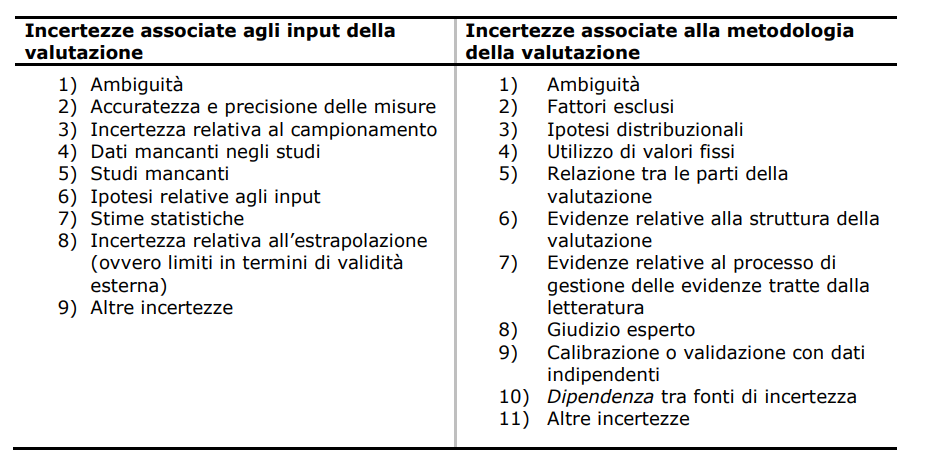
\includegraphics[width=0.9\columnwidth]{tipologia-incertezze} 
    \caption{Natura dell'incertezza}
\end{figure}

\subsubsection{Definizione delle priorità delle incertezze}

Definire le priorità delle fonti di incertezza è utile in diverse fasi della valutazione. All'inizio, aiuta a selezionare le incertezze più importanti per un'analisi approfondita. Durante la valutazione, individua le aree in cui cercare più dati o coinvolgere ulteriori esperti. Alla fine, identifica potenziali aree di ricerca futura. Le priorità dovrebbero basarsi sul contributo di ciascuna fonte di incertezza all'incertezza complessiva della valutazione, tenendo conto della dimensione dell'incertezza e della sua influenza sul risultato.
L'influenza delle diverse incertezze può essere valutata utilizzando giudizi esperti e scale ordinali. Si possono utilizzare metodi come le “tabelle d'incertezza” o l'approccio NUSAP.

Quando si usano modelli quantitativi, l'analisi di sensibilità può valutare l'influenza delle incertezze sugli input del modello. Le scelte riguardanti la struttura del modello possono essere verificate ripetendo la valutazione con alternative.

Per affrontare l'incertezza in modo efficace, è fondamentale che la valutazione sia suddivisa in parti principali, come esposizione e pericoli in una valutazione del rischio chimico, e in parti minori, come singoli parametri o studi. Questa suddivisione consente di eseguire l'analisi dell'incertezza a diversi livelli: valutare tutte le incertezze collettivamente, suddividerle in parti principali e combinarle successivamente, o suddividerle ulteriormente in parti più piccole e combinarle gradualmente. È essenziale combinare le parti dell'analisi per caratterizzare l'incertezza complessiva, definendo in anticipo come queste parti verranno integrate. Utilizzare un diagramma di modello concettuale può migliorare la trasparenza e il rigore del processo.\\

L'efficienza e l'affidabilità della valutazione dipendono dal livello di suddivisione scelto. Trattare separatamente le parti con incertezze rilevanti è generalmente più affidabile, mentre valutare tutte le incertezze collettivamente può essere più rapido ma meno preciso. Alcune incertezze minori possono essere considerate in una fase successiva della caratterizzazione complessiva, mentre quelle maggiori dovrebbero essere combinate tramite calcoli per garantire maggiore affidabilità. Quando si utilizzano modelli quantitativi, è utile quantificare l'incertezza per ciascun parametro e considerare anche le incertezze non quantificate, come quelle relative alla struttura del modello.\\

Per valutare correttamente l'incertezza, è essenziale che le domande e le quantità d'interesse siano chiaramente definite. Qualsiasi ambiguità aggiunge ulteriore incertezza e complica la valutazione. Se una domanda o quantità non è già ben definita, i valutatori devono provvedere a farlo per l'analisi dell'incertezza. Una quantità o domanda è ben definita se i valutatori possono concordare sulla risposta. Per ottenere ciò, si può specificare un esperimento, uno studio o una procedura che determinerebbe la risposta. Ad esempio, una misura ben definita per una quantità d'interesse dovrebbe includere specifiche di tempo, popolazione, luogo e condizioni. Allo stesso modo, la presenza o assenza di condizioni o meccanismi specifici deve essere dettagliata, così come i risultati di uno studio scientifico o un calcolo rilevante per la valutazione. Durante la formulazione delle domande, è importante identificare e sostituire termini ambigui o soggetti a giudizio di gestione del rischio con termini più chiari o numeri. Se i termini di riferimento sono aperti, è necessario che le conclusioni siano riferite a quantità ben definite o contengano affermazioni chiare e ben definite, necessarie per valutare ed esprimere l'incertezza associata.\\

L'espressione qualitativa dell'incertezza utilizza parole o categorie ordinali, senza quantificare le possibili risposte o probabilità. Questo metodo è utile in varie situazioni, come la definizione delle priorità delle incertezze e la descrizione di singole fonti di incertezza durante l'analisi. Le espressioni qualitative sono utili per definire le priorità, descrivere singole fonti di incertezza come passaggio preliminare per la quantificazione complessiva, comunicare i risultati usando una scala di probabilità approssimata con descrittori qualitativi, descrivere incertezze non incluse nella valutazione quantitativa e per la reportistica quando richiesto da decisori o normative.\\

Per descrivere singole fonti di incertezza, si raccomanda l'uso di scale ordinali per migliorare coerenza e trasparenza. Queste scale dovrebbero essere parte della pianificazione della valutazione e possono variare in formalità a seconda delle necessità. Le espressioni qualitative dovrebbero essere usate per elaborare un giudizio quantitativo sull'impatto combinato delle incertezze, basandosi su una logica chiara e non su calcoli arbitrari.\\

\subsection{Quantificare l'incertezza tramite probabilità}

Il Comitato scientifico raccomanda di esprimere quantitativamente l'impatto combinato delle incertezze. Le probabilità, specificate completamente o parzialmente, possono essere derivate da dati o giudizio esperto.\\

\textbf{Probabilità:} La probabilità varia da 0 a 1, espressa come percentuale da 0\% a 100\%. Per una domanda sì/no, 0\% significa che la risposta è sicuramente negativa, 100\% che è sicuramente positiva, e valori intermedi rappresentano vari gradi di certezza.\\

\textbf{Distribuzioni di probabilità:} L'incertezza relativa a una quantità non variabile può essere espressa tramite una distribuzione di probabilità, mostrando la probabilità relativa di diversi valori. Un'espressione parziale dell'incertezza può indicare la probabilità che un intervallo di valori includa il valore reale.\\

\textbf{Uso dei dati:} Quando disponibili, i dati dovrebbero essere utilizzati tramite analisi statistica, anche se il giudizio esperto interviene sempre, ad esempio nella scelta del modello  statistico. L'incertezza può essere quantificata direttamente o tramite calcoli dopo aver quantificato singole fonti di incertezza.\\



\section{Intelligenza artificiale in ambito medico: cosa ne pensano gli utenti nel 2024}

Secondo una recente indagine\footcite{womak:intelligenza-artificiale-e-medicina} dell'EngageMinds HUB, il Centro di ricerca dell'Università Cattolica, gli italiani ad oggi segnalano fiducia e timori verso l'uso dell'intelligenza artificiale in ambito medico.\\
Dal loro studio emerge che 6 italiani su 10 sono favorevoli all'uso dell'Intelligenza artificiale in ambito sanitario, di questi, l'88\% la userebbe per semplificare il linguaggio dei referti, l'86\% come supporto al medico per effettuare una diagnosi e l'80\% come aiuto per stabilire una terapia farmacologica adeguata, mentre quasi 6 italiani su 10 la utilizzerebbero come strumento per un'autoanalisi.\\
Di opinione meno positiva sono 7 italiani su 10 secondo i quali l'AI potrà causare una perdita della relazione e del contatto diretto con il medico.\\

Tra le principali opportunità che l'uso delle tecnologie digitali potranno portare, poco meno di 8 italiani su 10 (78\%) riferiscono che esse porteranno ad una maggiore accessibilità nell'accesso e nell'uso dei servizi, una riduzione dello spreco di carta e un maggior coinvolgimento del paziente grazie ad una maggiore accessibilità al proprio fascicolo sanitario. Il 74\% crede che le AI potranno ridurre i costi a lungo termine; poco meno di 7 su 10 ritengono che possa esserci un miglioramento nei monitoraggi tramite devices (68\%), mentre poco più di 6 su 10 si aspetta che le AI possano migliorare le diagnosi (63\%). Il 68\% degli italiani ritiene che l'uso di tecnologie digitali possano migliorare il monitoraggio da
remoto.\\

Un ulteriore rischio che gli italiani percepiscono è legato ai dati sensibili: per il 63\% l'uso dell'Intelligenza Artificiale potrà causare delle problematiche legate alla gestione della privacy, mentre per il 60\% legate alla diffusione di dati sensibili.
